\documentclass[11pt]{article}
\usepackage[utf8]{inputenc}
\usepackage[spanish,es-tabla]{babel}
\usepackage{amsmath}
\usepackage{amsfonts}
\usepackage{amssymb}
\usepackage{graphicx}

\usepackage{color, colortbl}

\usepackage{hyperref}
\usepackage{float}
\usepackage[a4paper,top=1.5cm,bottom=1.5cm,left=1.5cm,right=1.5cm,marginparwidth=1.75cm]{geometry}

\definecolor{LightYellow}{RGB}{217, 177, 85}

\title{Tubbing S.A \\ \small{Comunicaciones digitales} \\ \small{Universidad Nacional del Comahue} }
\author{ 
        Gatica, Isaias \\ \small{LautaroAndresSaez@gmail.com} \and 
        Millain, Gonzalo \\ \small{gonza.pm@outlook.com} \and
        Saez, Lautaro Andres \\ \small{IsaiasGatica1@gmail.com} 
}

\date{}

\begin{document}
    \maketitle
    \section{Generalidades}
    
        \subsection{Estructuras de redes}
        \begin{figure}[H]
            \centering
            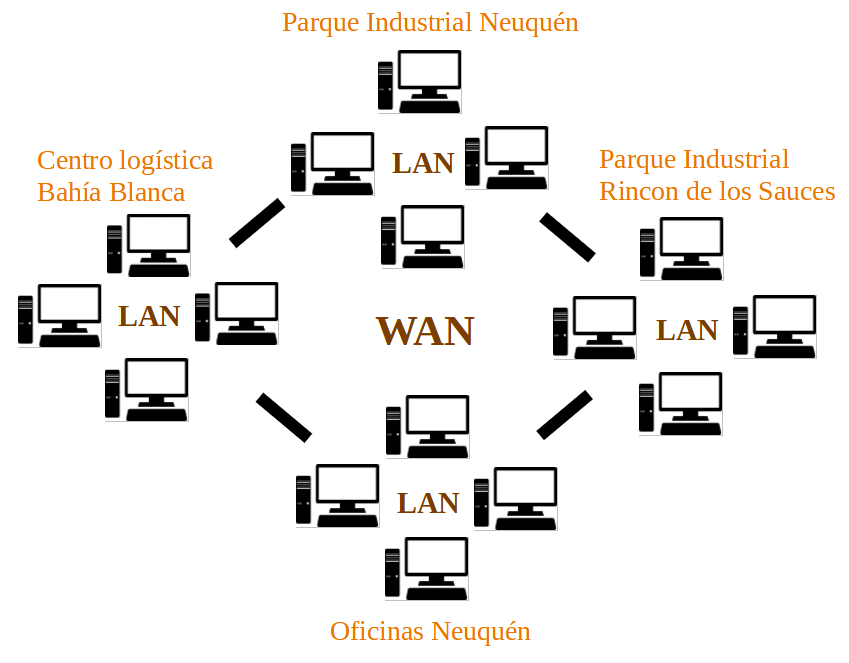
\includegraphics[scale=0.5]{Figure/Tubbin_Estructura.PNG}
            \caption{Imagen representativa de la estructura de Red}
            \label{Estructura}
        \end{figure}


        \subsubsection*{LAN}

        Cada área tendrá su propia red LAN, la cual mas adelante se definirá si será por cable o Wi-Fi dependiendo de las 
        prestaciones necesarias para cada lugar. Como primer medida adoptaremos el protocolo Ethernet por ser el mas utilizado.

        \subsubsection*{WAN}

        Se tendrá una red WAN que realice una interconexión entre todas las áreas con la central que estará ubicada en Parque Industrial.
        Esto permitirá mediante una red Proxy/VPN facilitando el teletrabajo.

        \subsubsection*{Seguridad}

        Para aumentar la seguridad de la red WAN/LAN y tener un mayor control del uso de la red y quienes usan dicha red 
        se decide implementar un servidor Proxy y/o un VPN.

        \subsection{Servicios de terceros}

        Debido a la complejidad de montar algunos sistemas y costo que esto conlleva se decidió tomar servicios de terceros, los 
        cuales se nombran a continuación.

        \subsubsection*{Servidor remoto}

        Con la finalidad de disminuir el costo de mantenimiento de un servidor y los cambios en la infraestructura que esto llevaría se 
        alquilara un servidor. Los precios de estos servidores rondan entre los $\$5000$ y $\$20000$ por mes, en este 
        caso nos decantaríamos por un servicio intermedio el cual cuesta $\$6000$. El proveedor es \href{https://www.hostdime.com.ar/servidores-dedicados}{\textit{hostdime}}.

        \subsubsection*{Flota de camiones}

        Dada la importancia de realizar un seguimiento de la flota de camiones y el bajo costo de alquilar un servicio.
        Tomando como referencia $\$800$ por camión del servicio \href{https://galileosatelital.com/rastreo-vehicular-gps}{\textit{Galileo}}.
        
    \section{Diseño de redes LAN}

    \subsection{Parque Industrial}

        Del proveedor de internet se conecta directamente un cable a los switch a utilizar. 

        Los Switch a utilizar serán $2$ \href{https://articulo.mercadolibre.com.ar/MLA-714545399-switch-cisco-semi-admin-24-puertos-10100-2-giga-sf220-24-k9-_JM#position=34&type=item&tracking_id=4df4b6b4-1084-45cf-bab2-a07d312cf877}{\textit{Cisco SF220-24-K9}}
        cuyo precio ronda lo $\$18000$.


        Se deciden armar las siguientes VLAN's: 

        \begin{enumerate}
            \item Cámaras de seguridad: van a tener su propio dvr 
            \href{https://articulo.mercadolibre.com.ar/MLA-658975031-dvr-xvr-dahua-8ch-canales-hd-1080n-cooper-pentahibrido-p2p-_JM#reco_item_pos=0&reco_backend=machinalis-seller-items-pdp&reco_backend_type=low_level&reco_client=vip-seller_items-above&reco_id=5b1ef3a8-b109-48d2-8d27-f2781047b33d}{\textit{Dahua de 8 canales}}
            en el que guardar las grabaciones en discos rígidos. De éste aparato se conecta un cable al switch.
            \item Gerencia y reuniones y oficinas: Cuenta con una VLAN con VPN para evitar trafico no deseado.
            \item Laboratorio: Idem anterior.
            \item Refrigerios y limpieza: El cual lleva una red Wi-Fi sin VPN para que los empleados puedan entrar a redes sociales, y 
                consumir contenido multimedia. Para esto se utilizará una access point económico.
                Se utilizara un access point 
                \href{https://www.mercadolibre.com.ar/access-point-router-tp-link-archer-c80-negro-1-unidad/p/MLA15904250?pdp_filters=category:MLA430901%7CCONNECTION_TYPE:279958#searchVariation=MLA15904250&position=2&type=product&tracking_id=d8d0e6d5-6d3c-4d79-9478-ce1d3aa1232d}{\textit{tp-link}}.
            \item Planta industrial: Para lograr una interconexión entre los PLC's.
        \end{enumerate}

        \begin{figure}[H]
            \centering
            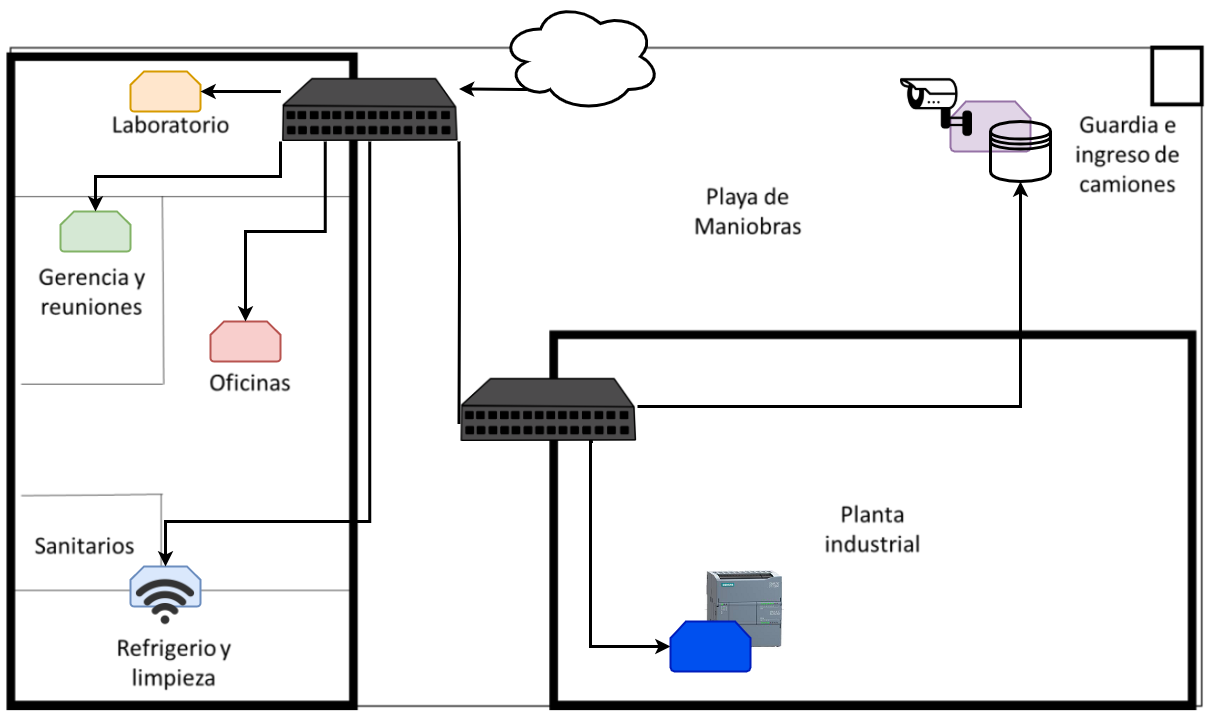
\includegraphics[width=\textwidth]{Figure/Planta_de_parque.png}
            \caption{Imagen ilustrativa de la estructura de Red del Parque Industrial. Cada trapecio de distinto color indica una VLAN diferente.}
        \end{figure}
        

    \subsection{Parque industrial Rincón de los Sauces}

    Se utiliza un switch Cisco SF220-24-K9. Y se implementaran las siguientes VLAN's: 

    \begin{enumerate}
        \item Cámaras de seguridad: Al igual que en parque central se utilizara un dvr 
        \href{https://articulo.mercadolibre.com.ar/MLA-658974667-nvr-dvr-dahua-4-canales-penta-hdcvi-xvr-1a04-5-ch-5x1-qr-ps2-_JM#position=1&type=item&tracking_id=c1ba311d-e835-4420-9ba9-f01382834064}{\textit{Dahua 4 canales}} e ira conectado por un cable al switch principal.
        \item Oficinas: Cuentan con su propia VLAN con VPN.
        \item Instrumentos: Cuentan con una VLAN cableada con VPN.
        \item Refrigerio, limpieza y sanitarios: Red Wi-Fi sin VPN con access point tp-link. 
    \end{enumerate}

    \begin{figure}[H]
        \centering
        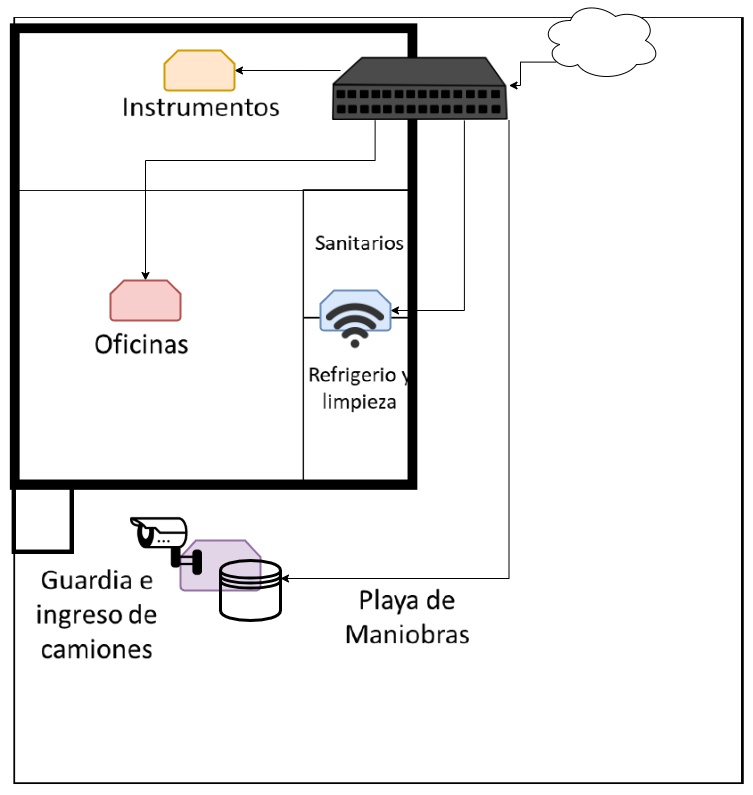
\includegraphics[width=0.6\textwidth]{Figure/Parque_Industrial.png}
        \caption{Imagen ilustrativa de la estructura de Red de la planta de Rincón de los Sauces. Cada trapecio de distinto color indica una VLAN diferente.}
    \end{figure}

    \subsection{Oficinas comerciales Neuquén}

    En esta oficina se utilizaran dos access point para garantizar las conexiones y no tener que invertir en cableado. Se utilizará un access point 
    \href{https://www.mercadolibre.com.ar/access-point-interior-ubiquiti-networks-unifi-ac-lr-ap-uap-ac-lr-blanco-1-unidad/p/MLA7953376?pdp_filters=category:MLA1700#searchVariation=MLA7953376&position=1&type=product&tracking_id=933ff74a-93c5-4a58-9a31-9fe5a3c5746e}{\textit{Ubiquiti Unifi Uap-lr}}
    por cada piso.

    \begin{figure}[H]
        \centering
        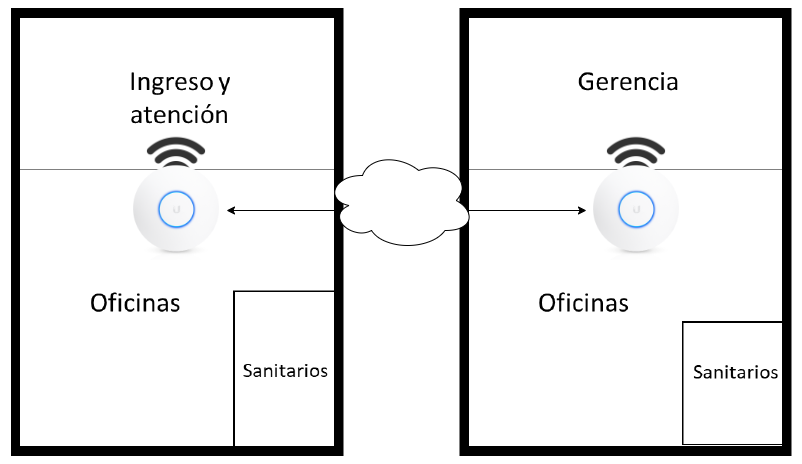
\includegraphics[width=0.6\textwidth]{Figure/Centrales_Neuquen.png}
        \caption{Imagen ilustrativa de la estructura de Red de las oficinas comerciales.}
    \end{figure}

    \subsection{Centro de logística Bahía Blanca}
    Se utiliza la misma idea de para las cámaras de seguridad de parque industrial y al ser pocas personas la conectividad será directamente del router/modem 
    del proveedor de internet. De esta forma se evita comprar un switch. 
    
    \begin{figure}[H]
        \centering
        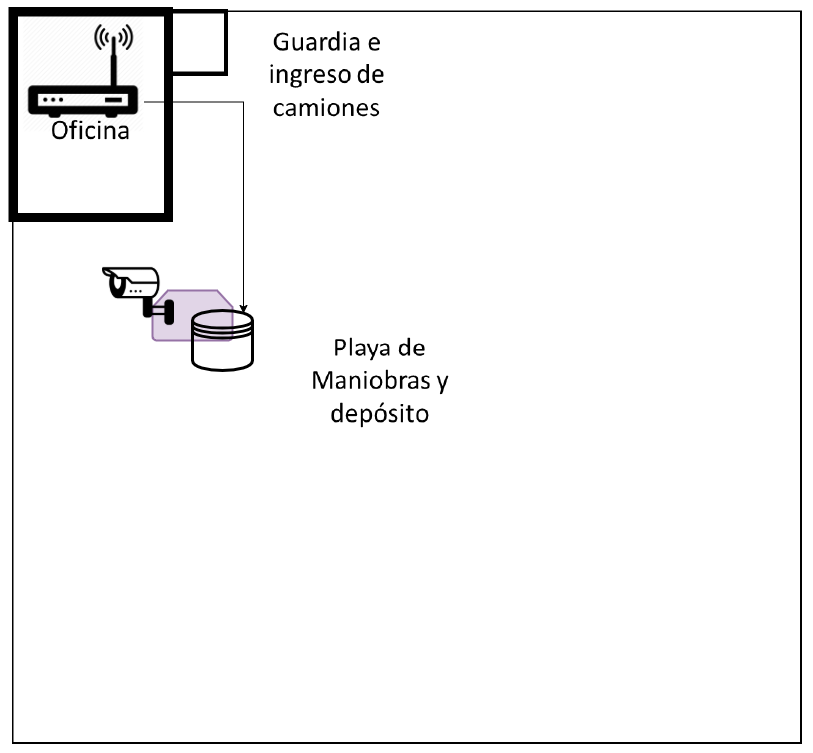
\includegraphics[width=0.6\textwidth]{Figure/Central_Bahia.png}
        \caption{Imagen ilustrativa de la estructura de Red del centro de Bahía Blanca.}
    \end{figure}

    \section{Diseño de redes IP}

    La numeración a implementar para las redes IP es 192.168.X y se utilizara siempre la mascara 255.255.255.0, donde X será un número identificatorio de cada sucursal.

    \begin{table}
        \centering
        \begin{tabular}{|c|c|c|}
    \hline Sucursal & IP & Mascara \\
    \hline Parque industrial & 192.168.1.0 & 255.255.255.0 \\ 
    \hline Oficina & 192.168.2.0 & 255.255.255.0 \\  
    \hline Parque industrial Rincón de los Sauces  & 192.168.3.0 & 255.255.255.0 \\
    \hline Centro de logística Bahía Blanca & 192.168.4.0 & 255.255.255.0 \\     
    \hline
\end{tabular}
        \caption{Numeración de las redes IP para cada sucursal.}
    \end{table}


    \section{Cableado}

    A continuación se muestras las tablas para cada sucursal, se recomienda tercerizar el servicio de instalación a \href{https://blgnet.com.ar/home/index.php#contact}{BLGNET}.

    \subsection{Parque industrial}

    \begin{table}[H]
        \centering
        \begin{tabular}{|c|c|c|c|}
            \hline Nombre & Modelo & Cantidad & Precio por unidad [u$\$$d] \\ 
            \hline Switch Cisco & Sf220-24-k9 & 2 & $225$ \\
            \hline Patchera 24 puertos & - & 2 & $100$ \\ 
            \hline Cable utp 6 & - & - & $1.75$ por metro  \\
            \hline Roseta & - & 30 & $3$  \\
            \hline
        \end{tabular}
    \end{table}
    
    \subsection{Parque industrial Rincón de los Sauces}

    \begin{table}[H]
        \centering
        \begin{tabular}{|c|c|c|c|}
            \hline Nombre & Modelo & Cantidad & Precio por unidad [u$\$$d] \\ 
            \hline Switch Cisco & Sf220-24-k9 & 1 & $225$ \\
            \hline Patchera 24 puertos & - & 1 & $100$ \\ 
            \hline Cable utp 6 & - & - & $1.75$ por metro  \\
            \hline Roseta & - & 10 & $3$  \\
            \hline
        \end{tabular}
    \end{table}
    
    \subsection{Oficinas comerciales Neuquén}

    \begin{table}[H]
        \centering
        \begin{tabular}{|c|c|c|c|}
            \hline Nombre & Modelo & Cantidad & Precio por unidad [u$\$$d] \\  
            \hline Cable utp 6 & - & - & $1.75$ por metro  \\
            \hline Access point Ubiquiti & AC LR AP & 2 & $168.6$\\
            \hline
        \end{tabular}
    \end{table}

    \subsection{Centro de logística Bahía Blanca}

    \begin{table}[H]
        \centering
        \begin{tabular}{|c|c|c|c|}
            \hline Nombre & Modelo & Cantidad & Precio por unidad [u$\$$d] \\  
            \hline Cable utp 6 & - & - & $1.75$ por metro  \\
            \hline Roseta & - & 3 & $3$  \\
            \hline
        \end{tabular}
    \end{table}


    \section{WAN}
    Con la finalidad de otorgar un servicio estable y profesional, se buscará contratar la red WAN a tercero, en específico una SD-WAN que es la tecnología mas actual. Si bien en Argentina aun no se encuentra variedad de prestadores, la mejor opción que se presenta es la de \textbf{Telefónica}.

        \subsection{SD-WAN Telefónica}
        Entre las opciones, se eligió la \href{https://empresas.telefonica.com.ar/cloud-computing/sdwan/sdwan}{Advantage SD - WAN Avanzado} por su no limitación en la cantidad de VLAN y la topología Full Mesh. Además incluye las características del plan básico como QoS, ruteo por aplicación o en seguridad IPSEC entre otras características. 
        En cuanto a la configuración para cada capa se propone:
        \begin{itemize}
            \item El protocolo de enrutamiento elegido es \textbf{Enrutamiento dinámico por estado de enlace}
            \item El control de congestión que se propone es el \textbf{Control por admisión} negociando un acuerdo entre el host y la subred de los parámetros de transmisión.
            \item En cuanto a la calidad de servicio QoS se utilizará la técnica de \textbf{Modelado de tráfico} y tratando de implementar a su vez la técnica de \textbf{Reservación de recursos}.
        \end{itemize}

    \section{Aplicaciones}
    
        \subsection{DNS}
        Podemos registrar un nombre de dominio \textit{.ar} por medio de \href{https://nic.ar/es/dominios/aranceles}{NIC Argentina}.

        %Aca tendriamos que mover el tema del hosting de la pagina web (servidor remoto). Ver el tema del mantenimiento de la misma, si se va a utilizar para contenido estatico o dinamico.

        \subsection{Email}
        Se busco un proveedor de correo, con posibilidad de utilizar nuestro nombre de dominio personalizado. Se eligió \href{https://www.microsoft.com/es-ar/microsoft-365/business}{Microsoft 365 para empresas}, este nos permite otras soluciones de almacenamiento de archivos y de otras aplicaciones varias.

        \subsection{Telefonia IP}
        Para la adquisión de telefonia IP en la empresa, se decidió optar por el servicio de \textit{IPTEL}. En particular nos decantamos por la
        \href{https://www.iptel.com.ar/centrales-telefonicas/virtuales/}{telefonia IP virtual} ya que nos da las mismas funcionalidades que una físca y además obtenemos
        características importantes como:
        \begin{itemize}
            \item Escalabilidad
            \item Ahorro económico
            \item Movilidad
            \item Internos remotos (Softphone)
        \end{itemize}

        Se eligío esta empresa por ser Argentina y contar con licencia de la CNC (Comisión Nacional de Comunicaciones).

    \section{Seguridad}
    %Que se necesita en terminos de seguridad al utilizar sdwan (ya tengo IPsec bajo sdwan)
    %Poner aca lo del servidor local para autenticacion (Uno por cada LAN, excepto tal vez BahiaBlanca)
    En términos generales de seguridad se seguirán las estrategias propuestas por la bibliografía. Estas son incluir:
    \begin{itemize}
        \item Firewall
        \item VPN
        \item IPSEC con ESP (\textit{Encapsulating Security Payload}) en modo tunel.
    \end{itemize}

    Actualmente el contratar un buen Firewall nos da la posibilidad de configurar los restantes items entre muchas otras ventajas. Por esto veremos a continuación tres Firewall
    recomendados para empresas: \footnote{https://tecnoloco.istocks.club/los-mejores-firewalls-para-pequenas-empresas-en-2020/2020-02-01/}

    \begin{enumerate}
        \item  \href{https://www.ui.com/edgemax/edgerouter/}{Ubiquiti EdgeRouter}: Si bien no es un Firewall en si, este router tiene prestaciones de seguridad que apuntan a pequeñas
        empresas. Se podría clasificar como un Firewall simple, aun así al ser de \textit{Ubiquiti} no da seguridad y por lo visto en su web proporciona 
        un control intuitivo y completo con aplicaciones web o de celular.
        \item \href{https://meraki.cisco.com/lib/pdf/meraki_datasheet_mx_es.pdf}{Meraki MX}: Ya un Firewall mas profesional y con la garantia de ser de Cisco es la gama de Meraki MX.
        Como vemos en el datasheet asociado, existen varios modelos en que se diferencian principalmente por la cantidad de interfaces LAN/WAN, el rendimiento en seguridad y firewall, la
        cantidad de VPN concurrentes y el tipo de montaje. 
        \item \href{https://www.fortinet.com/content/dam/fortinet/assets/white-papers/wp-security-fabric.pdf}{Fortinet Security Fabric}: Similar al Firewall de Cisco, muy profesional y
        en líderes de seguridad en la red como Fortinet. Las especificaciones son muy similares al anterior y tambien varían segun las características anteriores. Sin embargo, un apartado 
        intersante es la implementación de inteligencia artificial para mejorar la seguridad.
    \end{enumerate}

    Cabe destacar que tanto los Firewall de Cisco como los de Fortinet, en particular el modelo 
    \href{https://www.fortinet.com/content/dam/fortinet/assets/data-sheets/FortiGate_80E_Series.pdf}{FortiGate 80E} permiten configurar una SD-WAN. Esto nos brinda la 
    posibilidad de unificar los servicios y prescindir del servicio elegido anteriormente de Telefónica. En este punto nosotros proponemos....

    \section{Presupuesto}

    \begin{table}[H]
        \centering
        \begin{tabular}{|c|c|c|c|}
    \hline Nombre & Modelo & Cantidad & Precio [u$\$$d] \\ 
    \hline Servidor dedicado & Single Xeon quad-core & 1 & $128.75$ \\ 
    \hline Rastreador satelital & Galileo & - & $11.25$ \\
    \hline Switch Cisco & Sf220-24-k9 & 3 & $225$ \\
    \hline Dvr Dahua & DH XVR 1A08 & 1 & $100$ \\ 
    \hline Dvr Dahua & XVR 1A04 & 2 & $68.75$ \\ 
    \hline Access point tp-link & C80 & 2 & $71.25$ \\ 
    \hline Access point Ubiquiti & AC LR AP & 2 & $168.6$\\

    \rowcolor{LightYellow}
    \hline \multicolumn{3}{|c|}{Total} & $1520.95$\\
    \hline
    
\end{tabular}
        \caption{Presupuesto tentativo en dólares (17/11/2020).}
    \end{table}

    \end{document}
